\documentclass[11pt,a4paper]{article}
\usepackage{od}
\usepackage[utf8]{inputenc}
\usepackage[english]{babel}
\usepackage{tikz}
\usetikzlibrary{shapes.misc}
\usetikzlibrary{arrows.meta}

\pagestyle{headings}
\title{TRIZ-Summit Cup – 2019/2020}

\author{The official English version, moved to \LaTeX\ by Hans-Gert Gräbe,
  Leipzig .}

\date{November 10, 2019}

\newcommand{\video}{Videos should be short (from 2 to 5 minutes). All authors
  of the given video should be mentioned: screenplay writer, film editor,
  actors, etc.
  
  This work is directed at forming methodological material for TRIZ teaching.
  
TRIZ Summit web-site\footnote {\url
  {http://triz-summit.ru/en/contest/competition/video/}, \\ \url
  {https://www.youtube.com/channel/UCjMNOjboWRBQA72DJvaC7ew/featured}}
contains videos, presented to the last TRIZ Summit Cup.

Tasks for TRIZ Summit Cup-2018/2019 were prepared by M.S. Rubin, N.V. Rubina
nomination «fantasizing» was prepared by P.R. Amnuel.
}

\newcommand{\melies}{
\begin{minipage}{.6\textwidth}
  \paragraph{1.}
  The founder of the genre of science-fiction film is the French filmmaker
  George Méliès. Each of more than 500 short-length films shot by Méliès, are
  distinguished by inimitable «filmmaker’s mannerism». While shooting the film
  «A visit to the wreckage of cruiser «Man» (1897--1898) it was necessary to
  show a distinct picture of people working under water in the episode «divers
  at work», and also a distinct picture of wreckage of the cruiser. Underwater
  photography existed in those times, however, they were looked upon as
  something exotic: sufficiently good quality could not be attained even in a
  rather transparent water. For example, look at one of the first photographs
  made under water, made in France in 1893 (we hope, you’ll agree that the
  quality is insufficient for a film). How did they manage to shoot a good
  quality underwater sequence?
\end{minipage} \hfill
\begin{minipage}{.35\textwidth}
  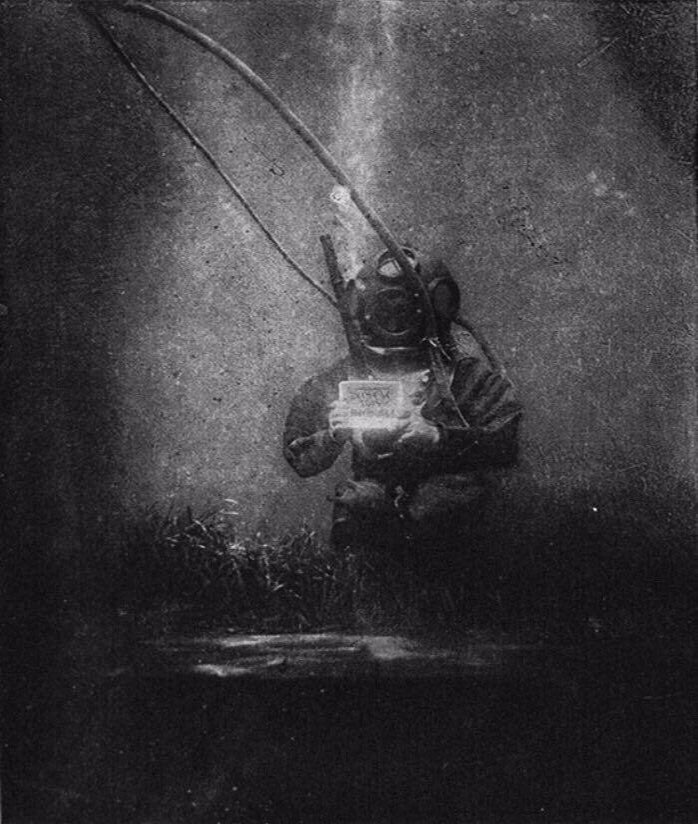
\includegraphics[width =\textwidth]{Bild-1.jpg}
\end{minipage}
\medskip

The film by George Méliès «In the Kingdom of
Fairies»\footnote{\url{https://www.youtube.com/watch?v=paM_BPyRT1o&t=542s}}
uses a similar effect.  It is surprising, but the same special effect was used
by the filmmaker Alexander Ptushko in the screened fairy tale «Sadko» in
sequences, where the action takes place at the bottom of the sea, in the realm
of the Sea King.

What other special effects are used in cinema and for solving what problems
are they used? What contradictions appear thereby and what techniques are used
for resolving these contradictions?
}

\newcommand{\hollywood}{
\paragraph{2.}
In the history of the biggest corporate film company – Hollywood – there are
episodes, which are associated neither with the creative process, nor with the
invention of new technical means for film-making, but with a purely law
problem.  By the turn of the 20$^\mathrm{th}$ century the man, who possessed
main patents for film-making equipment was Thomas Edison (that very inventor
of a filament lamp). However, the majority of film-makers of that time were
main owners of independent companies. Besides, they all worked with equipment,
which they themselves improved and adapted to making films based on their own
ideas. Because of that they did not consider it to be necessary to pay
interest to Edison for using his patents. On December 18, 1908 Edison
announced the creation of Motion Picture Patents Company (MPPC), which entered
the history of cinema as the Edison Trust. Several film companies entered this
Trust, but the majority preferred to remain independent. The day of December
24, 1908, when the jurisdiction of the Trust entered into force, became known
in the history of American cinematography  as «black Christmas». According to
the rules introduced by Edison, independent companies had to pay the Trust
huge amounts of money for their right to shoot and demonstrate films. The
police closed 500 out of 800 film theaters in New York at the pretext of
violation of patent rights. What decision did the independent companies take,
in order not to depend upon Edison Trust?

Do you know of any examples of commercial marketing solutions, which
contributed to the evolution of film art or braked it?  }

\newcommand{\kinogenres}{
\paragraph{1.}
What genres of cinema do you know? Create the chronology of origination of
different genres of the cinema. Is it possible to use the examples of genres
of film art for illustrating the Lines of system evolution, known in TRIZ (for
example, dynamization, mono-bi-poly-trimming, transition to micro-level)? What
genres of film art do you like best of all and why?

\paragraph{2.}
In film history there are people whose achievements and contribution to the
development of cinema are rather significant, while their names are forgotten.
Collect information concerning the biographies of these film-makers. What
problems did they solve and what techniques did they use?  What do you think,
what Qualities of a Creative Personality helped them to achieve their goals?
Often, having solved a particular problem the person stops and, being
satisfied with his achievements, cannot create anything new.  It is
surprising, but the company of Lumière brothers, who have entered history as
creators of cinematography, creased to produce films in 1900, only 5 years
after the first commercial show of films on December 28, 1895 – the birthday
of cinema. What do you think, what can be an obstacle for a person in
attainment of significant results in creative activity?}

\newcommand{\kinotools}{
\paragraph{1.}
Select several techniques, which are used by film directors, cameramen, sound
engineers and screenplay writers (editing, pauses, special effects,
slow-motion and quick-motion shooting, etc.) for obtainment of certain effects
in cinema. Use these techniques in your videos. Describe your idea in greater
detail in the description accompanying the video. Is it possible to intensify
these effects using TRIZ methods?

\paragraph{2.}
Videos on history of photography, cinema and inventions, which were made in
these fields.  }

\newcommand{\contradictions}{ In creating an animated cartoon film it is
  necessary to resolve several contradictions:
\begin {itemize}
\item The number of drawings of which the film consists, should be as large as
  possible, so that the picture should be continuous, without jumps, and it
  should be as small as possible, in order to reduce time for creating an
  animated cartoon film.
\item The drawings, of which the cartoon film consists, should have the
  largest possible number of details, so that the characters should be
  emotional, and should contain the smallest number of details in order to
  facilitate the process of creating the animated cartoon film.
\item The camera filming individual drawings, should be immobile, so that the
  picture should be distinct and include the objects, which gradually change
  their position, and should be mobile, in order to include different shooting
  angles and different volume of space, surrounding the object.
\end{itemize}
How were these contradictions solved in different techniques of creating
animated cartoon films?
}

\begin{document}
\maketitle

\section{Category: 8--10 years }

\subsection*{Nomination «Inventive activity»}

\paragraph{1.}
\contradictions

\paragraph{2.}
G.S. Altshuller in his book «Find the idea» proposed a method of creating
plots for an animated cartoon film (or a tale), which could be called «Fairy
Tales with contradictions». An algorithm for creating such a tale (a plot for
an animated cartoon film) is as follows:
\begin{enumerate}
\item Select a character or an object of a fairy tale plot
\item Imagine the environment of the character in a nutshell.
\item Apply the technique of fantasizing (increase, decrease, do-it-reverse,
  animate, imagination binomial, etc.). 
\item Formulate an anti-idea and contradiction. Create a plot based on solving
  of this contradiction. 
\item Introduce a restriction or create a new contradiction in the plot using
  cl. 3. Solutions of the contradiction-development of plot.
\item The result is a very fast moving plot.
\end{enumerate}
Invent a plot for an animated cartoon film, using this algorithm.

\subsection*{Nomination «Fantasizing»}

\paragraph{1.}
In 1974 American science fiction author James Teeptry wrote a story «The girl,
who was plugged in». There is such an episode in this story: the film is
projected with the aid of lasers to the clouds above the city and all
citizens, looking upwards, can watch the film. Nowadays it almost ceased to be
science fiction – laser shows on the clouds have become popular. However,
these are not exactly films. Invent a new fantastic method for demonstrating
films.

\paragraph{2.}
Soviet science fiction author Nickolay Vassilenko in his story «The Curved
mirror» (1977) described a fantastic mirror: when a person looks into it, he
sees not the reflection, but a small film, in which the essence of the human
being, who looks into the mirror, is presented in the image of a certain
animal. Write a science fiction story, based on this idea, however, change the
idea with the help of one of the techniques for fantasizing.

\subsection*{Nomination «TRIZ Tools»}

\paragraph{1.}
What elements does a cartoon camera consist of? In what way are they
interconnected? Which functions are played by each element? Of what materials
is it possible to manufacture characters of an animated cartoon film? Invent
your own character for an animated cartoon film and a small story about him.

\paragraph{2.}
Compile a collection of cards on using the techniques of fantasizing in
animated cartoon films and screen adaptations of fairy tales. Analyze this
collection of cards. What techniques are most often used for creating typical
characters or images (for example, imagine how the image of a curious,
mischievous and courageous Buratino is created: long (increased) nose seems to
be created «to be peeped into other people’s affairs»; «personalized» wood log
«does not drown in water and cannot be burnt by fire»). Compare, how similar
images are created in different animated cartoon films (screened fairy tales):
kind and evil magicians, hero warriors, beautiful princesses, capricious
princesses, etc. What is your favorite animated cartoon film? Which particular
episodes in this animated cartoon film do you like? Are any techniques for
fantasizing used in them?

\subsection*{Nomination «Research»}
Compile a collection of cards on inventors (or scientists) and their
inventions (discoveries). Analyze this cards collection. What problems are
solved by the characters of these animated cartoon films? What techniques were
used for solving problems? How are they found solutions (discoveries) used in
the life of people?

\subsection*{Nomination «TRIZ Videos»}
\kinotools

\video

\clearpage
\section{Category: 11--14 years}

\subsection*{Nomination «Inventive activity»}

\paragraph{1.}
In 1909 the American film-maker David Griffith shot a mute short film «Lonely
villa»\footnote{\url{https://www.youtube.com/watch?time_continue=13&v=5RdbnyNYAv8}}
(which lasted only 7 minutes). This is an action film about an attempt at
robbery of a lonely villa. Most probably, this was the first thriller movie
(action film causing tension and excitement with the spectator). Three points
of view are presented in this film:
\begin{itemize}
\item the family staying inside the house and trying to rescue from robbery;
\item the gangsters attacking a rich house;
\item  head of the family and policemen, which appear «at the last moment».
\end{itemize}
Griffith had an objective to show (during 7 minutes) the starting of this
story, penetration of gangsters into the house, the fear of the housewife and
her three daughters and (the most important) – the rescue. Prior to creation
of «Lonely villa» the films contained such plots, which embraced one event and
reflected the sequence of actions of the characters chronologically (the time
in the movie coincided with the time of the event in life). What’s to be done,
in order to show different lines of the plot during a short time and at the
same time to intensify the impression (tension) with the spectators? What film
technique did David Griffith use for the first time? What other film
techniques did Griffith invent and for the creation of what effects were they
used? Select a problem or several problems, which were solved by D. Griffith
and analyze them according to the following pattern: formulate contradictions,
IFR, enumerate resources, which are present in the problem, techniques for
resolving contradictions, which could be applied to this problem. Which
techniques of filming do you know and for the solving of what problems are
they used?

\paragraph{2.}
\contradictions

\subsection*{Nomination «Fantasizing»}

\paragraph{1.}
The American science fiction author Thomas Sherred in his story «The Attempt»
described a film, which was shot with the aid of a time machine. Invent a
fantastic method for creating films. How will the films be shot in future?

\paragraph{2.}
In the story «The Flying Eagle» by Pavel Amnuel (1970) a dramatist, inventing
the plot for a would-be play, does not write the text, as they do now, but
creates a video film, imagining that the play has already been staged. He does
not need actors, he himself plays the characters embodying their acting manner
and their behavior. Invent a story based on this new idea, but change it using
some technique of fantasizing.

\subsection*{Nomination «TRIZ Tools»}

Describe a technological operation principle of cinema. Of what parts does the
CINEMA consist? How do these parts interact for the purpose of obtainment of a
cinematographic effect? What effects (physical, chemical and physiological)
are used in film shooting and demonstration? How did perception and mentality
of people change during decades of existence of cinema? What do you think:
what effects will be used in the cinema in future?

\subsection*{Nomination «Research»}

\paragraph{1.}
What genres of cinema do you know? Create the chronology of origination of
different genres of the cinema. Is it possible to use the examples of genres
of film art for illustrating the Lines of system evolution, known in TRIZ (for
example, dynamization, mono-bi-poly-trimming, transition to micro-level)? What
genres of film art do you like best of all and why?

\paragraph{2.}
In 1927 the first show of the film «The Jazz
Singer»\footnote{\url{https://my.mail.ru/mail/wikki0508/video/5622/29304.html}}
took place. It was the first sound film in the history of cinematography. It
is difficult for a modern reader to imagine a film without words and sound
effects. However, by far not all the film-makers immediately accepted this
revolutionary change. «Muteness, two-dimensionality and monochrome nature of
the film are not its shortcomings, but its «structural essence». Film art does
not need to overcome them, since new expressive means will only hinder its
further improvement», -- that is what Yury Tynyanov wrote about peculiarities
of film art in 1930-ies. Try to prove the righteousness of opposing
viewpoints, first from the standpoint of those who oppose to introduction of
sound in the cinema, and then from the standpoint of followers of this
technology. What do you think: what new sound effects will appear in the film
art in future?

\subsection*{Nomination «TRIZ Videos»}
\kinotools

\video
\clearpage

\section{Category: 15--17 years}

\subsection*{Nomination «Inventive activity»}

\melies

\hollywood

\subsection*{Nomination «Fantasizing»}

\paragraph{1.}
A device is described in the novel by American science fiction author Philip
Dick «Do androids dream of electric
sheep?»\footnote{\url{http://lib.ru/INOFANT/DICKP/sheeps.txt}}, which enables
a group of people to experience feelings of a selected person and to perceive
the world in the same way as he perceives it.  Thus it is possible to shoot
films and the spectators will feel everything that the actor felt during the
shooting process. Invent a new fantastic idea, changing the idea of Dick with
the aid of a «staged matrix» of G.S. Altshuller.

\paragraph{2.}
Alexander Belyaev in his novel «The Ruler of the World»
(1929\footnote{\url{https://www.litmir.me/br/?b=3062&p=1}.}) described
«theater of thought», in which the actors don’t act on the stage, but only
imagine their acting, while the spectator «catches» these thoughts and
«watches» the performance mentally. Write a science fiction story about the
shooting of such a «thought-based film», changing the idea of Belyaev by using
one of the techniques of fantasizing.

\subsection*{Nomination «TRIZ Tools»}

It is possible to single out several Lines of development in the evolution of
technical systems, for example, «mono-bi-poly-trimming»; «dynamization»;
«emptiness»; «transition to microlevel»; «personal – personal-corporate –
corporate». Compile a collection of cards, illustrating these Lines of
development in the field of cinema or photography. Take into account that both
cinema and photography are at the same time art and production technology as
well as a commercial product (film theaters, advertizing, attending consumer
services, etc.).

\subsection*{Nomination «Research»}
\kinogenres

\subsection*{Nomination «TRIZ Videos»}
\kinotools 
\video
\clearpage

\section{Category: students}

\subsection*{Nomination «Inventive activity»}

\melies

\hollywood

\subsection*{Nomination «Fantasizing»}

\paragraph{1.}
In science fiction stories by the Japanese author Kobo Abe «Totaloscope» and
the Italian writer Lino Aldani «Onirofilm» (both stories were published in
1965) films are described, which were shot with the full participation effect
and feedback with the spectator.  Change this idea using such techniques of
fantasizing, using several techniques instead of one.  Describe the result.

\paragraph{2.}
The American science fiction author Frank Herbert in his space epic «The Dune»
(1965\footnote{\url{https://www.litmir.me/br/?b=196731&p=1}.}) described how
one of the characters controls the behavior of other characters using special
voice intonations. At that the person, who is being controlled, understands it
fairly well but cannot do anything: he has to obey. Think of a plot for an
adventure film of the future taking the idea of Herbert as a basis, but
changing it with the development of plot using the techniques of fantasizing.

\subsection*{Nomination «TRIZ Tools»}

Trends of technical systems evolution is the basis of TRIZ. There are several
possible classifications of these trends. We offer you one of such
classifications.

\begin{center}
\newcommand{\law}[2]{\parbox{#1cm}{\small\centering #2}}
\tikz[>={Triangle[length=3pt 9, width=3pt 3]}] {
  
\node[draw] at (5,7) [rectangle]
(A1) {\law{3}{Trend of increasing ideality}};

\node[draw] at (0,6) [rectangle]
(A2) {\law{4}{Trend of increasing completeness (Trend of completeness of
    performing operation)}};

\node[draw] at (0,2) [rectangle]
(A3) {\law{4}{Trend of increasing coordination of system parts}};

\node[draw] at (0,4) [rectangle]
(A4) {\law{4}{Trend of conductivity (of energy, flows, etc.)}};

\node[draw] at (5,5) [rectangle]
(A5) {\law{3}{Trend of irregular evolution of system parts}};

\node[draw] at (10,0) [rectangle]
(A6) {\law{4}{Tendency of system S-curve evolution}};

\node[draw] at (0,0) [rectangle]
(A7) {\law{4}{Tendency of elimination of human involvement}};

\node[draw] at (10,4) [rectangle]
(A8) {\law{4}{Trend of increasing controllability and Su-Field interactions}};

\node[draw] at (5,1) [rectangle]
(A9) {\law{3}{Trend of increasing dynamicity}};

\node[draw] at (5,3) [rectangle]
(A10) {\law{3}{Trend of transition to the super-system}};

\node[draw] at (10,6) [rectangle]
(A11) {\law{4}{Trend of transition from macro-level to micro-level}};

\node[draw] at (10,2) [rectangle]
(A12) {\law{4}{Tendency of system evolution due to trimming or ??}};

\draw[->] (A1) -- (2.8,7) |- (A2) ;
\draw[->] (2.8,7) |- (A3);
\draw[->] (2.8,7) |- (A4);
\draw[->] (2.8,7) |- (A5);
\draw[->] (2.8,7) |- (A7);
\draw[->] (2.8,7) |- (A9);
\draw[->] (2.8,7) |- (A10);
\draw[->] (A2) -- (-2.7,6) |- (A7);
\draw[->] (A5) -- (7.2,5) |- (A9);
\draw[->] (7.2,5) |- (A10);
\draw[->] (7.2,5) |- (A6);
\draw[->] (A1) -- (7.5,7) |- (A8) ;
\draw[->] (7.5,7) |- (A11) ;
\draw[->] (7.5,7) |- (A12) ;
\draw[->] (A8) -- (12.5,4) |- (A12) ;
}
\end{center}
Analyze the stages of cinematography evolution using the system of Trends of
Technical Systems Evolution. How can one forecast further development of film
art taking into account the tendencies in cinematography evolution?


\subsection*{Nomination «Research»}
\kinogenres
\subsection*{Nomination «TRIZ Videos»}
\kinotools

\video


\end{document}
